% @autor Ионкин Михаил
% Большая часть настроек взята с диплома БГУ ( Yury Yaroshevich. Диплом в LaTeX. URL: https://github.com/mstyura/bsuir-diploma-latex/tree/master/MiKTeX ). 
% Часть настроек взял из стиля, созданного Vladimir Protsenkovi (URL: https://github.com/protsenkovi/latex-ssau-gost-style).
% Добавил часть своих настроек, объединил существующие, внес исправления под стандарты СГАУ. Старался взять лучшее из этих проектов и других источников. 
% Использовал JabRef и KBibTeX для создания библиографического списка. 

\documentclass[a4paper,14pt,oneside,final]{extreport}

\usepackage[framemethod=default]{mdframed}
\usepackage{moreverb}

\usepackage{lastpage}
% Предоставляет проприетарный Times New Roman.
%\usepackage{pscyr}
% Выбор шрифта по-умолчанию. 
% Пункт 2.1.1 Требований по оформлению пояснительной записки.
% Примечание: В требованиях не указан, какой именно шрифт использовать. По традиции используем TNR.
%\renewcommand{\rmdefault}{ftm}
% Установка кодировки исходных файлов.
\usepackage[utf8]{inputenc}
% Учет особенностей различных языков.
\usepackage[russian]{babel}
% Выбор внутренней TeX кодировки.
\usepackage[T2A]{fontenc}
%Если планируете использовать Times New Romans (ftm), то нужно будет установить пакет PSCyr.
% PSCyr на Linux: http://plumbum-blog.blogspot.ru/2010/11/pscyr-tex-live.html?showComment=1290219013107#c2607271373129816963 (придется вспомнить команды копирования в терминале). На Windows инструкцию найти достаточно легко, как и исполнить её. 

% Делает результирующий PDF "searchable and copyable".
\usepackage{cmap}
% Чтобы можно было использовать русские буквы в формулах, но в случае использования предупреждать об этом.
\usepackage[warn]{mathtext}
% Зачем: Добавляет поддержу дополнительных размеров текста 8pt, 9pt, 10pt, 11pt, 12pt, 14pt, 17pt, and 20pt.
% Почему: Пункт 2.1.1 Требований по оформлению пояснительной записки.
\usepackage{extsizes}
% Зачем: Длинна, пимерно соответвующая 5 символам
% Почему: Требования содержат странное требование про отсупы в 5 символов (для немоноширинного шрифта :| )
\newlength{\fivecharsapprox}
\setlength{\fivecharsapprox}{5ex}
% Зачем: Добавляет отступы для абзацев.
% Почему: Пункт 2.1.3 Требований по оформлению пояснительной записки.
\usepackage{indentfirst}
\setlength{\parindent}{\fivecharsapprox} % Примерно соответсвует 5 символам.
% Зачем: Настраивает межстрочный интервал, для размещения 40 +/- 3 строки текста на странице.
% Почему: Пункт 2.1.1 Требований по оформлению пояснительной записки.
\usepackage[nodisplayskipstretch]{setspace} 
\setstretch{1.1}
% Зачем: Отключает использование изменяемых межсловных пробелов.
% Почему: Так не принято делать в текстах на русском языке.
\frenchspacing
% Сброс счетчика сносок для каждой страницы
% Примечание: в "Требованиях по оформлению пояснительной записки" не указано, как нужно делать, но в других БГУИРовских докуметах рекомендуется нумерация отдельная для каждой страницы
\usepackage{perpage}
\MakePerPage{footnote}
% Добавляет скобку 1) к номеру сноски
% Пункты 2.9.2 и 2.9.1 Требований по оформлению пояснительной записки.
\makeatletter \def\@makefnmark{\hbox{\@textsuperscript{\normalfont\@thefnmark)}}} \makeatother
% Зачем: Расположение сносок внизу страницы
% Почему: Пункт 2.9.2 Требований по оформлению пояснительной записки.
\usepackage[bottom]{footmisc}
% Переопределяем стандартную нумерацию, т.к. в отчете будут только section и т.д. в терминологии TeX
\makeatletter \renewcommand{\thesection}{\arabic{section}} \makeatother
% Зачем: Пункты (в терминологии требований) в терминологии TeX subsubsection должны нумероваться
% Почему: Пункт 2.2.3 Требований по оформлению пояснительной записки.
\setcounter{secnumdepth}{3}
% Зачем: Настраивает отступ между таблицей с содержанимем и словом СОДЕРЖАНИЕ
% Почему: Пункт 2.2.7 Требований по оформлению пояснительной записки.
\usepackage{tocloft}
\setlength{\cftbeforetoctitleskip}{-1em}
\setlength{\cftaftertoctitleskip}{1em}
% Определяет отступы слева для записей в таблице содержания.
% Пункт 2.2.7 Требований по оформлению пояснительной записки.
\makeatletter
	\renewcommand{\l@section}{\@dottedtocline{1}{0.5em}{1.2em}}
	\renewcommand{\l@subsection}{\@dottedtocline{2}{1.7em}{2.0em}}
\makeatother
% Задает стиль заголовков раздела жирным шрифтом, прописными буквами, без точки в конце
% Пункты 2.1.1, 2.2.5, 2.2.6 и ПРИЛОЖЕНИЕ Л Требований по оформлению пояснительной записки.
\makeatletter
\renewcommand\section{%
  \clearpage\@startsection {section}{1}%
    {\fivecharsapprox}%
    {-1em \@plus -1ex \@minus -.2ex}%
    {1em \@plus .2ex}%
    {\centering\hyphenpenalty=10000\normalfont\normalsize\bfseries\MakeUppercase}}
\makeatother


% Зачем: Задает стиль заголовков подразделов
% Почему: Пункты 2.1.1, 2.2.5 и ПРИЛОЖЕНИЕ Л Требований по оформлению пояснительной записки.
\makeatletter
\renewcommand\subsection{%
  \@startsection{subsection}{2}%
    {\fivecharsapprox}%
    {-1em \@plus -1ex \@minus -.2ex}%
    {1em \@plus .2ex}%
    {\raggedright\hyphenpenalty=10000\normalfont\normalsize\bfseries}}
\makeatother
% Зачем: Задает стиль заголовков пунктов
% Почему: Пункты 2.1.1, 2.2.5 и ПРИЛОЖЕНИЕ Л Требований по оформлению пояснительной записки.
\makeatletter
\renewcommand\subsubsection{
  \@startsection{subsubsection}{3}%
    {\fivecharsapprox}%
    {-1em \@plus -1ex \@minus -.2ex}%
    {\z@}%
    {\raggedright\hyphenpenalty=10000\normalfont\normalsize\bfseries}}
\makeatother
% Зачем: для оформления введения и заключения, они должны быть выровнены по центру.
% Почему: Пункты 1.1.15 и 1.1.11 Требований по оформлению пояснительной записки.
\makeatletter
\newcommand\sectioncentered{%
  \clearpage\@startsection {section}{1}%
    {\z@}%
    {-1em \@plus -1ex \@minus -.2ex}%
    {1em \@plus .2ex}%
    {\centering\hyphenpenalty=10000\normalfont\normalsize\bfseries\MakeUppercase}%
    }
\makeatother
% Зачем: Задает стиль библиографии
% Почему: Пункт 2.8.6 Требований по оформлению пояснительной записки.
\bibliographystyle{ugost2008}
% Зачем: Пакет для вставки картинок
% Примечание: Объяснение, зачем final - http://tex.stackexchange.com/questions/11004/why-does-the-image-not-appear
\usepackage[final]{graphicx}
\DeclareGraphicsExtensions{.pdf,.png,.jpg,.eps}
% Зачем: Директория в которой будет происходить поиск картинок
%\graphicspath{{/home/misha/latex/LR2Optics/LR2/}}
% Зачем: Добавление подписей к рисункам
\usepackage[nooneline]{caption}
\usepackage{subcaption}
% Зачем: чтобы работала \No в новых латехах
\DeclareRobustCommand{\No}{\ifmmode{\nfss@text{\textnumero}}\else\textnumero\fi}
% Зачем: поворот ячеек таблиц на 90 градусов
\usepackage{rotating}
\DeclareRobustCommand{\povernut}[1]{\begin{sideways}{#1}\end{sideways}}
% Зачем: Задание подписей, разделителя и нумерации частей рисунков
% Почему: Пункт 2.5.5 Требований по оформлению пояснительной записки.
\DeclareCaptionLabelFormat{stbfigure}{Рисунок #2}
\DeclareCaptionLabelFormat{stbtable}{Таблица #2}
\DeclareCaptionLabelSeparator{stb}{~--~}
\captionsetup{labelsep=stb}
\captionsetup[figure]{labelformat=stbfigure,justification=centering}
\captionsetup[table]{labelformat=stbtable,justification=raggedright}
\renewcommand{\thesubfigure}{\asbuk{subfigure}}

% Зачем: Окружения для оформления формул
% Почему: Пункт 2.4.7 требований по оформлению пояснительной записки и специфические требования различных кафедр
% Пример использования смотри в course_content.tex, строка 5
\usepackage{calc}
\newlength{\lengthWordWhere}
\settowidth{\lengthWordWhere}{где}
\newenvironment{explanationx}
    {%
    %%% Следующие строки определяют специфические требования разных редакций стандартов. Раскоменнтируйте нужную строку
    %% стандартный абзац, СТП-01 2010
    %\begin{itemize}[leftmargin=0cm, itemindent=\parindent + \lengthWordWhere + \labelsep, labelsep=\labelsep]
    %% без отступа, СТП-01 2013
    \begin{itemize}[leftmargin=0cm, itemindent=\lengthWordWhere + \labelsep , labelsep=\labelsep]%
    \renewcommand\labelitemi{}%
    }
    {%
    %\\[\parsep]
    \end{itemize}
    }

% Старое окружение для "где". Сохранено для совместимости
\usepackage{tabularx}
\newenvironment{explanation}
    {
    %%% Следующие строки определяют специфические требования разных редакций стандартов. Раскоменнтируйте нужные 2 строки
    %% стандартный абзац, СТП-01 2010
    \par 
    \tabularx{\textwidth-\fivecharsapprox}{@{}ll@{ --- } X }
    %% без отступа, СТП-01 2013
    %\noindent 
    %\tabularx{\textwidth}{@{}ll@{ --- } X }
    }
    { 
    \\[\parsep]
    \endtabularx
    }
% Зачем: Удобная вёрстка многострочных формул, масштабирующийся текст в формулах, формулы в рамках и др
\usepackage{amsmath}
% Зачем: Поддержка ажурного и готического шрифтов 
\usepackage{amsfonts}
% Зачем: amsfonts + несколько сотен дополнительных математических символов
\usepackage{amssymb}
% Зачем: Окружения «теорема», «лемма»
\usepackage{amsthm}
% Зачем: Производить арифметические операции во время компиляции TeX файла
\usepackage{calc}
% Зачем: Производить арифметические операции во время компиляции TeX файла
\usepackage{fp}
% Зачем: Пакет для работы с перечислениями
 \usepackage{enumitem}
 \makeatletter \AddEnumerateCounter{\asbuk}{\@asbuk}{щ)} \makeatother
% Зачем: Устанавливает символ начала простого перечисления
% Почему: Пункт 2.3.5 Требований по оформлению пояснительной записки.
 \setlist{nolistsep}
% Зачем: Устанавливает символ начала именованного перечисления
% Почему: Пункт 2.3.8 Требований по оформлению пояснительной записки.
\renewcommand{\labelenumi}{\asbuk{enumi})}
\renewcommand{\labelenumii}{\arabic{enumii})}
% Зачем: Устанавливает отступ от границы документа до символа списка, чтобы этот отступ равнялся отступу параграфа
% Почему: Пункт 2.3.5 Требований по оформлению пояснительной записки.
\setlist[itemize,0]{itemindent=\parindent + 2.2ex,leftmargin=0ex,label=--}
\setlist[enumerate,1]{itemindent=\parindent + 2.7ex,leftmargin=0ex}
\setlist[enumerate,2]{itemindent=\parindent + \parindent - 2.7ex}
% Зачем: Дополнительные возможности в форматировании таблиц
\usepackage{makecell}
\usepackage{multirow}
\usepackage{array}
% Зачем: "Умная" запятая в математических формулах. В дробных числах не добавляет пробел
% Почему: В требованиях не нашел, но в русском языке для дробных чисел используется {,} а не {.}
\usepackage{icomma}
% Зачем: макрос для печати римских чисел
\makeatletter
\newcommand{\rmnum}[1]{\romannumeral #1}
\newcommand{\Rmnum}[1]{\expandafter\@slowromancap\romannumeral #1@}
\makeatother
% Зачем: Управление выводом чисел.
\usepackage{sistyle}
\SIdecimalsign{,}
% Зачем: inline-коментирование содержимого.
\newcommand{\ignore}[2]{\hspace{0in}#2}
% Зачем: Возможность коментировать большие участки документа
\usepackage{verbatim}
\usepackage{xcolor}
% Зачем: Оформление листингов кода
% Примечание: final нужен для переопределения режима draft, в котором листинги не выводятся в документ.
\usepackage[final]{listings}
\usepackage[normalem]{ulem}

\usepackage{url}
\usepackage[final,hidelinks]{hyperref}
% Моноширинный шрифт выглядит визуально больше, чем пропорциональный шрифт, если их размеры одинаковы. Искусственно уменьшаем размер ссылок.
\renewcommand{\UrlFont}{\small\rmfamily\tt}

\usepackage[square,numbers,sort&compress]{natbib}
\setlength{\bibsep}{0em}

% Магия для подсчета разнообразных объектов в документе
\usepackage{lastpage}
\usepackage{totcount}
\regtotcounter{section}

\usepackage{etoolbox}

\newcounter{totfigures}
\newcounter{tottables}
\newcounter{totreferences}
\newcounter{totequation}

\providecommand\totfig{} 
\providecommand\tottab{}
\providecommand\totref{}
\providecommand\toteq{}

\makeatletter
\AtEndDocument{%
  \addtocounter{totfigures}{\value{figure}}%
  \addtocounter{tottables}{\value{table}}%
  \addtocounter{totequation}{\value{equation}}
  \immediate\write\@mainaux{%
    \string\gdef\string\totfig{\number\value{totfigures}}%
    \string\gdef\string\tottab{\number\value{tottables}}%
    \string\gdef\string\totref{\number\value{totreferences}}%
    \string\gdef\string\toteq{\number\value{totequation}}%
  }%
}
\makeatother

\pretocmd{\section}{\addtocounter{totfigures}{\value{figure}}\setcounter{figure}{0}}{}{}
\pretocmd{\section}{\addtocounter{tottables}{\value{table}}\setcounter{table}{0}}{}{}
\pretocmd{\section}{\addtocounter{totequation}{\value{equation}}\setcounter{equation}{0}}{}{}
\pretocmd{\bibitem}{\addtocounter{totreferences}{1}}{}{}

% Для оформления таблиц не влязящих на 1 страницу
\usepackage{longtable}

% Для включения pdf документов в результирующий файл
\usepackage{pdfpages}
% Для использования знака градуса и других знаков
% http://ctan.org/pkg/gensymb
\usepackage{gensymb}
% Зачем: преобразовывать текст в верхний регистр командой MakeTextUppercase
\usepackage{textcase}
% Зачем: Переносы в словах с тире.
% Тире в словае заменяем на \hyph: аппаратно\hyphпрограммный.
% https://stackoverflow.com/questions/2193307/how-to-get-latex-to-hyphenate-a-word-that-contains-a-dash#
\def\hyph{-\penalty0\hskip0pt\relax}
\usepackage{amsmath}
\usepackage{amsfonts}
\usepackage{amssymb}
\usepackage{graphicx}
\usepackage{lmodern}
% поля
\usepackage[left=3cm,right=1.5cm,top=2cm,bottom=2cm]{geometry}
% толерантность к переносам
\tolerance 6000%
% для списка источников
\makeatletter \renewcommand{\@biblabel}[1]{\stepcounter{totreferences}#1 \hfill} \makeatother
% для случая, когда документ маленький, и всего одна секция
%\renewcommand{\thesection}{}
%\renewcommand{\thesubsection}{\arabic{subsection}}
%\renewcommand{\thesubsubsection}{\arabic{subsection}.\arabic{subsubsection}}
% не помню зачем. Кажется, разреживает таблицу.
\renewcommand{\arraystretch}{1.5}

\renewcommand{\rmdefault}{cmr} % Шрифт с засечками
\renewcommand{\sfdefault}{cmss} % Шрифт без засечек
\renewcommand{\ttdefault}{cmtt} % Моноширинный шрифт
\renewcommand{\labelitemi}{--}
\renewcommand{\labelenumi}{\theenumi.}

\usepackage{chngcntr}
\counterwithin{equation}{section}

\usepackage{indentfirst}
\usepackage{cool}
\usepackage{commath}

\newcommand*\rfrac[2]{{}^{#1}\!/_{#2}}
\DeclareMathAlphabet{\mathpzc}{OT1}{pzc}{m}{it}
\newcommand{\z}{\mathpzc{z}}
\usepackage{mathtools}

\usepackage{hyperref}
\hypersetup{colorlinks = true}
% для правильной и быстрой записи дифференциалов и частных производных
\usepackage{physics}
\allowdisplaybreaks
%\displaybreak[0]
% http://tex.stackexchange.com/questions/42271/floor-and-ceiling-functions
\usepackage{mathtools}
\DeclarePairedDelimiter{\ceil}{\lceil}{\rceil}

\usepackage{amsmath}
\usepackage{tcolorbox}

\usepackage{listings}

\usepackage{color}
\definecolor{dkgreen}{rgb}{0,0.6,0}
\definecolor{gray}{rgb}{0.5,0.5,0.5}
\definecolor{mauve}{rgb}{0.58,0,0.82}
\definecolor{deepblue}{rgb}{0,0,0.5}
\definecolor{deepred}{rgb}{0.6,0,0}
\definecolor{deepgreen}{rgb}{0,0.5,0}

% Default settings for code listings
\lstset{frame=tb,
  aboveskip=3mm,
  belowskip=3mm,
  showstringspaces=false,
  columns=flexible,
  basicstyle=\renewcommand{\baselinestretch}{0.95}\ttfamily,
  numbers=none,
  numberstyle=\tiny\color{gray},
  keywordstyle=\bfseries\color{orange!40!black},
  commentstyle=\itshape\color{purple!40!black},
  identifierstyle=\color{black},
  emph={Main,MyMath, Data, Solution, 
  		Int, Double, String, Array, Unit,
  		Console, math},          % Custom highlighting
  emphstyle = \color{deepgreen},    % Custom highlighting style
  stringstyle=\color{mauve},
  frame=L,
  xleftmargin=\parindent,
  breaklines=true,
  breakatwhitespace=true
  tabsize=3
  framexleftmargin=8mm, 
  rulesepcolor=\color{blue},
}

\begin{document} 	  
	\begin{titlepage}
  \begin{center}
			МИНИСТЕРСТВО ОБРАЗОВАНИЯ И НАУКИ \\ РОССИЙСКОЙ ФЕДЕРАЦИИ 
			\vspace{0.5cm}
			\linebreak  ФЕДЕРАЛЬНОЕ ГОСУДАРСТВЕННОЕ АВТОНОМНОЕ \\
			ОБРАЗОВАТЕЛЬНОЕ УЧРЕЖДЕНИЕ ВЫСШЕГО ОБРАЗОВАНИЯ	\\
			«САМАРСКИЙ ГОСУДАРСТВЕННЫЙ АЭРОКОСМИЧЕСКИЙ \\
			УНИВЕРСИТЕТ ИМЕНИ АКАДЕМИКА С.\,П. КОРОЛЕВА \\
			(НАЦИОНАЛЬНЫЙ ИССЛЕДОВАТЕЛЬСКИЙ УНИВЕРСИТЕТ)» (СГАУ) 
			%\hrulefill
		\vspace{0.25cm} \\
		\begin{large}
			Факультет информатики \\
			Кафедра технической кибернетики\\	
		\end{large} 
		\vspace{1cm} 
		Расчётно-пояснительная записка к курсовой работе\\
		по дисциплине <<Уравнения математической физики>> 
		\vspace{1.5cm} \\
		\begin{large}
		Тема: 	 \textbf{<<\textsc{аналитическое решение краевых задач  математической физики}>>}
		\end{large}		
		\vspace{1cm} \\ 
		Вариант №\,5
	\end{center}
	\vspace{3cm} 
		\begin{tabular}{ll}
		Выполнил студент & Ионкин М.\,A. \\ 
		Группа & 6407 \\ 
		Руководитель работы & Быков Д.\,А. 
		\end{tabular} 	
	\vspace{\fill}
	\begin{center}
		САМАРА 2015
	\end{center}
\end{titlepage} 
	\setcounter{page}{2}
	\section*{Задание}
%\addcontentsline{toc}{section}{Задание}
\label{sec:solve}
   	Решить задачу теплопроводности на сфере радиуса~$R$. Нагревание происходит за счет поглощения энергии излучения полусферой (см. рис.~\ref{fig:sphere}), причем количество поглощённой энергии определяется косинусом угла между нормалью и направлением распространения излучения. 

   	При моделировании использовать следующую математическую модель:  	
   	\begin{equation}
   		\label{eq: init_equation}
   		\begin{cases}
    	c \pderiv{u}{t} = K \triangle u + \beta f (\overrightarrow{r}),    
    	      \quad  \{x \in   \mathbb{R}^3 \mid \rho(x,0) = R\}, t\geqslant 0; \\
    	u(\theta,\rho,t) \big|_{t=0} = 0.
    	\end{cases}
	\end{equation}  
\begin{explanationx}
	\item[где] $u(\theta, \varphi,t)$ --- функция, описывающая температуру в некоторой точке $(R,\theta,\varphi)$ в момент времени $t$; 
	\item $f$ --- функция, описывающая энергию, поглощенную единицей площади;
	\item $c$ --- положительная константа; 
	\item $K$ --- положительная константа.
\end{explanationx} 

	\begin{figure}[hb!]
 		\begin{center}
 			\includegraphics{/home/misha/latex/EMF/the-3dplot-package.pdf}
			\caption{К условиям задачи}
	 		\label{fig:sphere}
 		\end{center}
	\end{figure} 	
	
	В данной курсовой работе необходимо:
	\begin{enumerate}
	\item Используя метод разделения переменных, получить решение задачи математической физики в виде ряда Фурье.
	\item Исследовать сходимость ряда. Получить оценку остатка ряда. 
	\item Разработать программу расчёта решения задачи с требуемой точностью. (Если необходимо, то использовать метод численного интегрирования для расчёта коэффициентов ряда. При этом следует контролировать погрешность численного интегрирования.)   
	\item Исследовать качество полученной аналитической оценки остатка ряда, используя вычислительный эксперимент. 
	\end{enumerate}
	\section*{Реферат} 

Отчет \pageref*{LastPage} с,  \totfig{}~рисунка, \toteq{} уравнений, 7~использованных источников. %, \toteq{}~формул и . \total{section}~раздел,%\pageref{LastPage}

\begin{large}
\textsc{уравнения математической физики, уравнение теплопроводности, полиномы лежандра, разложение в ряд}
\end{large}
	
	Целью данной работы является решение задачи теплопроводности на шаре при заданных параметрах, более конкретно --- разработка программы, выводящей график зависимости температуры от координат шара, времени и заданных констант. 
	
	Программа разрабатывалась в операционной системе \textit{Ubuntu 15.10} с использованием сред  \textit{Scala IDE}, \textit{Netbeans} и  \textit{IntelliJ Idea Community Edition}. 
\newpage 
	% Зачем: Содержание пишется полужирным шрифтом, по центру всеми заглавными буквами
% Почему: Пункт 2.2.7 Требований по оформлению пояснительной записки.
\renewcommand \contentsname {\centerline{\bfseries\normalsize{\MakeUppercase{содержание}}}}
% Зачем: Не захламлять основной файл
% Примечание: \small\selectfont злостный хак, чтобы уменьшить размер шрифта в ToC 
{
\normalsize\selectfont
\tableofcontents
%\newpage
}
	\section*{Введение}
% http://tex.stackexchange.com/questions/74439/table-of-contents-incorrect-page-numbering
\phantomsection
\addcontentsline{toc}{section}{Введение}
\label{sec:intro}

В данной работе решается задача теплопроводности на сфере. Изменение температуры происходит за счет поглощения энергии верхней полусферой --- аналогичная ситуация возникает, например, при нагреве Солнцем поверхности Земли.

В первом разделе исходная задача сводится к разложению искомой функции в ряд по ортогональным функциям --- полиномам Лежандра. Это позволяет рассматривать счетное множество независимых уравнений. В конце раздела приводится явное разложение функции температуры, что позволяет найти решение в численном виде. 

Во втором разделе проверяется сходимость ряда и оценивается его остаток в зависимости от количества слагаемых ряда. В результате, можно по заранее заданной точности определить число слагаемых, а значит --- решить задачу с заданной точностью с использованием ЭВМ. 

В третьем разделе приводится код программы, необходимый и достаточный для вычисления функции температуры. В нем же указывается ссылка на полный код проекта (а также на \textit{jar}-архив), скомпилировав (запустив) который можно просматривать график решения. В конце раздела приводятся примеры графиков при заданных параметрах.  
   	
	\section{Представление решения в виде ряда}
	\subsection{Упрощение модели}	
	Оператор Лапласа в сферических координатах задается уравнением 
	\begin{equation}
   	\label{eq: Laplass_share_basic}
   	\triangle u(r,\theta,\varphi,t) = \frac{1}{r^2} \pdv{}{r} \left( r^2 {\pdv{u}{r}} \right) + \frac{1}{r^2 \sin \theta} \pdv{}{\theta} \left( \sin \theta {\pderiv{u}{\theta}} \right) + \frac{1}{r^2\sin^2 \theta} {\partial^2 u \over \partial \varphi^2} .
	\end{equation}
	
	В нашем случае, $r$ является константой $(r \equiv R)$. Также, можно выбрать базис (систему координат) так, чтобы функция $u$ зависела лишь от одного пространственного параметра, а именно, от $\theta$ (как это показано на рис. \ref{fig:sphere}). 
	Поэтому оператор Лапласа можно записать в следующем виде: 
	\begin{equation}
   	\label{eq: my_Laplas_share}
   	\triangle u(\theta,t) = \frac{1}{R^2 \sin \theta} \pdv{}{\theta} \left( \sin \theta {\pderiv{u}{\theta}} \right).
	\end{equation}
	
	Таким образом, из уравнений (\ref{eq: init_equation}) и (\ref{eq: my_Laplas_share}) получаем, что 
	\begin{equation}
   	\label{eq: init_equation_before_decomposition}
   	c \pderiv{u}{t} = \frac{K}{R^2}\times\frac{1}{\sin \theta} \pdv{}{\theta} \left( \sin \theta \pderiv{u}{\theta} \right) + \beta f (\overrightarrow{r}).
	\end{equation} 
	Введем теперь замену $ u(t,\theta)=X(\theta)T(t) $:
	\begin{equation}
   	\label{eq: u=XT }
	c X(\theta) \dv{T}{t} = \frac{K}{R^2} T(t) \frac{1}{\sin \theta} \dv{}{\theta} \left( \sin \theta \dv{X}{\theta} \right) + \beta f (\overrightarrow{r}).
	\end{equation} 
	
	\subsection{Решение однородного уравнения}
	Рассмотрим однородное уравнение~(\ref{eq: u=XT }): 
	\begin{equation}
   	\label{eq: uniform}
   	c X(\theta) \dv{T}{t} = \frac{K}{R^2} T(t) \frac{1}{\sin \theta} \dv{}{\theta} \left( \sin \theta \dv{X}{\theta} \right), 
   	\end{equation} 	
	или
	$$ c \dv{\ln{T}}{t} = \frac{K}{R^2}\times\frac{1}{{X(\theta) \sin \theta}} \dv{}{\theta} 
	\left( \sin \theta \dv{X}{\theta} \right). $$
	
	Согласно  \cite[стр. 50]{Kyznetcov04MMF}, т. к. $\theta \text{ и } t$ --- независимые переменные, то  
	$$ \od{\ln{T}}{t} = \frac{K}{cR^2}\times\frac{1}{{X(\theta) \sin \theta}} \dv{}{\theta} 
	\left( \sin \theta \dv{X}{\theta} \right) = -\mu,$$ 
	\begin{explanationx}
		\item[где] $\mu$ --- некоторая константа. 
	\end{explanationx}  
	Следовательно, мы имеем два дифференциальных уравнения: 
		\begin{align}
		\label{eq:sol_decomp_1}
			\dv{\ln{T}}{t} + \mu &=0, \\
		\label{eq:sol_decomp_2}		
			 \dv{}{\theta}\left( \sin \theta \dv{X}{\theta} \right) 
			+ \mu \frac{cR^2}{K}  \sin \theta X &= 0.
		\end{align}
			
	Введем замену $x = \cos(\theta)$ и будем учитывать, что $\theta \in (0;\pi)$. Тогда
	$$ \dd{x} = -\sin(\theta)\dd{\theta}, \quad \dv{\theta} = -\sin(\theta) \dv{x} = -\sqrt{1-x^2}\dv{x}, $$
	 и	уравнение~(\ref{eq:sol_decomp_2}) преобразуется в 
	$$
		\dv{x}\left( -(1-x^2) \dv{X}{x} \right) - \mu \frac{cR^2}{K} X = 0,
	$$
	или
	\begin{equation}
		\label{eq:solution_hypergeimetrix_type}
		(1-x^2)\dv[2]{X}{x} - 2x \dv{X}{x} + \mu \frac{cR^2}{K} X = 0.
	\end{equation}
	
	Это есть уравнение гипергеометрического типа~(\cite[с. 12]{SpecFuncMF}). 
	Введем новые функции: $ \sigma(x) = 1-x^2 $, $ \tau(x) = -2x$, $\lambda = \mu \frac{cR^2}{K}$. Имеем:
	\begin{equation}
		\label{eq:solution_hypergeimetrix_type_2}
		\sigma(x)\od[2]{X}{x} + \tau(x)\od{X}{x} + \lambda X = 0.
	\end{equation}
	Для этого уравнения строится класс наиболее простых решений --- классические ортогональные полиномы, определяемые формулой Родрига~\cite[\S\,9 п.\,2]{SpecFuncMF}:
	\begin{equation}
		\label{eq:solution_Rodrigues_equation}
		y_n (x) = \frac{Y_n}{\rho(x)}\od[n]{}{x}\left[ \sigma^n \rho(x) \right], \qquad \forall n \in \mathbb{N}_0,
	\end{equation}
	\begin{explanationx}
		\item[где] $\rho(x)$ --- функция, удовлетворяющая уравнению $ (\sigma \rho )' = \tau \rho$;
		\item $\{Y_n\}$ --- некоторые константы.
	\end{explanationx} 
	При этом коэффициенты $ \lambda $  уравнения~(\ref{eq:solution_hypergeimetrix_type_2}), связаны соотношением $$ \lambda + n\tau ' + \rfrac{1}{2}n(n-1)\sigma '' = 0.$$
	
	В нашем случае, для нахождения множества коэффициентов получаем уравнения 
	\begin{equation} 
		\label{eq:solution_lambda_n}
		\lambda_n = n(1+n), \qquad \forall n \in \mathbb{N}_0. 
	\end{equation}
	
	Согласно~\cite[часть~II, \S\,1 п.\,3]{TihonovAndSamarskiy99EMF}, полиномы Лежандра $ \left\lbrace  P_n (x) \right\rbrace  $ являются собственными функциями оператора~$ \dv{x}\left((1-x^2) \dv{}{x} \right) $, соответствующие (биективно по эквивалентному номеру) полученным собственным значениям~$\left\lbrace  \lambda_n  \right\rbrace.$
	
	Используя полученные собственные функции  $ \left\lbrace  P_n (x) \right\rbrace  $, полная система которых одновременно является базисом для разложения других функций, мы можем записать функцию $ X $ через ряд:
	\begin{equation}
		\label{eq:solution_X_from_Legandr}
		X(x) = \sum_{k=0}^{+\infty} {B_k P_k (x)}.
	\end{equation}
	Возвращаясь к переменной $\theta$, получаем: 
	\begin{equation}
		\label{eq:solution_X_from_Legandr_withTheta}
		X(\theta) = \sum_{k=0}^{+\infty} {B_k P_k (\cos\theta)}.
	\end{equation}
	
	В то же время, по уравнению~(\ref{eq:sol_decomp_1}), с учетом полученных в системе~(\ref{eq:solution_lambda_n}) собственных чисел, можно определить функции 
	\begin{equation}
	\label{eq:solution_T_n} T_n(t) = e^{-\mu_n t} = e^{-n(1+n)\frac{K}{cR^2} t}, \qquad \forall n \in \mathbb{N}_0,
	\end{equation}   
	причем каждый $T_n, \; n \in \mathbb{N}_0,$ будет соответствовать $X_n$. Решениями уравнения~(\ref{eq:sol_decomp_1}), вообще говоря, являются функции $\{C_n T_n(t)\}$, где $\{C_n\}$ --- некоторое множество констант.
	
	Таким образом, мы можем разложить функцию $ u(t,\theta)=X(\theta)T(t)$ в ряд: 
	\begin{equation} 
		\label{eq:solution_u_via_sum}
u(t,\theta)=\sum_{k=0}^{+\infty}{C_k T_k(t)B_k P_k(\cos\theta)}=\sum_{k=0}^{+\infty}{A_k T_k(t)P_k (\cos\theta)} .
	\end{equation}
		
	\subsection{Решение неоднородного уравнения}
	Пусть функция $f$ уравнения~(\ref{eq: init_equation}) разлагается в ряд по полученным собственным функциям: 
	$$ f(\theta) =  \sum_{k=0}^{+\infty} {f_k P_k(\cos\theta)},$$
	при этом коэффициенты $ \left\lbrace f_k \right\rbrace $ находятся из условия ортогональности полиномов Лежандра:
	\begin{equation}
	\begin{split}
	\int_{-1}^{1}{f(\theta)P_n (\cos\theta) \dd{\cos\theta}} 
		&= \sum_{k=0}^{+\infty} \int_{-1}^{1}{f_k P_k (\cos\theta)P_n (\cos\theta)} \dd{\cos\theta} = \\
		&= {\left\Vert P_n  \right\Vert}^2 f_n, \qquad \forall n \in \mathbb{N}_0. 
	\end{split}
	\end{equation}	
	Таким образом, 
	\begin{equation}
	\label{eq: f_n}
		f_n = \frac{1}{{\left\Vert P_n  \right\Vert}^2}\int_{-1}^{1}{f(\theta)P_n (\cos\theta) \dd{\cos\theta}}, \qquad \forall n \in \mathbb{N}_0. 
	\end{equation}	
	
	Будем находить функцию $u$, используя метод вариации произвольных постоянных $\{A_k\}$: $\forall k \in \mathbb{N}_0 \; A_k = A_k(t)$. В соответствии с уже полученным разложением~(\ref{eq:solution_u_via_sum}), уравнение~(\ref{eq: init_equation_before_decomposition}) 
можно переписать в виде 
	\begin{multline}
	\label{eq: solution_dif_eq_withSum}
   	c \sum_{k=0}^{+\infty} {  P_k (\cos\theta)\dv{A_k T_k}{t}} = \\ =\frac{K}{R^2}\times\frac{1}{\sin \theta} \dv{}{\theta} \left( 
   				\sin \theta \sum_{k=0}^{+\infty} { A_k T_k\dv{ P_k (\cos\theta)}{\theta}}
   	 \right) 
   	+ \beta \sum_{k=0}^{+\infty} {f_k P_k(\cos\theta)}.
	\end{multline}
	
   	Очевидно, что если
   	\begin{equation}
   	\label{eq: solution_dif_eq_foreach}
   	\begin{split}	
   	c  { P_k (\cos\theta)\dv{A_k T_k}{t}} =& A_k T_k\frac{K}{R^2}\times\frac{1}{\sin \theta} \dv{}{\theta} \left( 
   				\sin \theta  { \dv{ P_k (\cos\theta)}{\theta}}
   	 \right) + \\
   	&+ \beta {f_k P_k(\cos\theta)}, \qquad \forall k \in \mathbb{N}_0,
	\end{split}   	
   	\end{equation}
   	то равенство в уравнении~(\ref{eq: solution_dif_eq_withSum}) будет выполняться.
   	
    Т.к. $\{P_k\}$ --- собственные функции оператора ~$ \dv{x}\left((1-x^2) \dv{}{x} \right) $, то
   	$$ \frac{1}{\sin\theta}\dv{}{\theta} \left( \sin \theta  { \dv{P_k (\cos\theta)}{\theta}}\right) = -\lambda_k  P_k (\cos\theta), $$ 
   	и из системы~(\ref{eq: solution_dif_eq_foreach}) получаем
   	$$
   	c  { P_k (\cos\theta)\dv{A_k T_k}{t}} = -  \lambda_k  P_k (\cos\theta) A_k T_k\frac{K}{R^2}  
    + \beta {f_k P_k(\cos\theta)}, \qquad \forall k \in \mathbb{N}_0, 	
   	$$
 или 
 	\begin{equation}
 	\label{eq: dif_eq_with_A_k(t)T_k(t)}
   	\dv{A_k T_k}{t} = - k(k+1) \frac{K}{cR^2}  A_k T_k  
    + \beta \frac{f_k }{c}, \qquad \forall k \in \mathbb{N}_0.
   	\end{equation}
   	
   	Решие уравнения $y' = - ay + b$ при $a \neq 0$ есть $ y = \frac{b}{a}+Ce^{-at}$, где $C$ --- некоторая константа. Поэтому решения системы~(\ref{eq: dif_eq_with_A_k(t)T_k(t)}) есть 
   	\begin{equation}
   	A_k(t) T_k =  
   	\begin{cases}
	    \frac{\beta \frac{f_k }{c}}{k(k+1) \frac{K}{cR^2}} + D_k T_k 
	    = \frac{\beta f_k}{k(k+1)}\times\frac{R^2}{K} + D_k T_k, & \forall k \in \mathbb{N}, \\
   	 	f_k\frac{\beta}{c}t + D_k, & k = 0,
   	 \end{cases}
   	 \end{equation}
   	 \begin{explanationx}
	\item[где] $\{D_k\}$ --- некоторое множество констант.
   	 \end{explanationx}
    Тогда из уравнения~(\ref{eq:solution_u_via_sum}) следует, что $u(\theta,t)$ есть
   	\begin{equation}
   	\label{eq: u_sum_over_D_k}
     \begin{split}
   	 u(\theta,t) =& \left( f_k \frac{\beta}{c}t + D_0 \right) P_0(\cos\theta) + \\
   	 &+\sum_{k=1}^{+\infty}{\left( 
   	 \frac{R^2}{K}\times\frac{\beta f_k}{k(k+1)} + D_k T_k(t)
		\right) P_k(\cos\theta)
   	 }.
   	  \end{split} 
   	 \end{equation}
	Применим однородное условие~(\ref{eq: init_equation}):
	\begin{equation}
		D_k =  
		\begin{cases}
			-\frac{R^2}{K}\times\frac{\beta f_k}{k(k+1)}, & \forall k \in \mathbb{N}, \\
			0, & k = 0.
		\end{cases}
	\end{equation}
	С учетом этого условия, окончательно получаем, что 
	\begin{equation}
   	\label{eq: u_final_sum_without_f_k}
   	 \begin{split}
   	 u(\theta,t) =  
   	 \beta \frac{R^2}{K}\sum_{k=1}^{+\infty}{
	   		 \frac{f_k}{k(k+1)}\left(1 - e^{-k(1+k)\frac{K}{cR^2} t}
		 \right)P_k(\cos\theta)} + \\
	 + f_0 \frac{\beta}{c} P_0(\cos\theta) t.
   	  \end{split} 
   	 \end{equation}
   	 
   	\subsection{Определение вида коэффициентов разложения $\{f_k\}_{0}^{+\infty}$ функции $f$}
   	    Согласно формулировки задания, функция $f(\theta)$ будет определяться из уравнения 
    \begin{equation}
    	f(\theta) = \eta(cos(\theta))\cos\theta ,
    \end{equation}  
     \begin{explanationx}
	\item[где] $\eta(x)$ --- функция Хевисайда.
   	 \end{explanationx}
    
    
	Определим теперь по формуле~(\ref{eq: f_n}) коэффициенты $\{f_k\}$: 
	\begin{equation}
	\label{eq: f_k_over_intsfP}
	\begin{split}
		f_k = &\frac{1}{\norm{P_k}^2}\int_{0}^{1}{\cos\theta P_k (\cos\theta) \dd{\cos\theta}} \\ 
			= &\frac{1}{\norm{P_k}^2}\int_{0}^{1}{xP_k(x)\dd{x}}, \qquad \forall k \in \mathbb{N}_0.
	\end{split}	
	\end{equation} 
	Норма $\norm{P_k}$, для всех $k\in \mathbb{N}_0$, согласно~\cite[часть II, \S\,1 п.\,5]{TihonovAndSamarskiy99EMF} определяется из уравнения
	\begin{equation}
	\label{eq: normPk}
	\norm{P_k} = \sqrt{\frac{2}{2n+1}}.
	\end{equation} 
	
	Согласно~\cite[ур-е 26]{LegendreRochester}, для всех целых $n>1$ 
	\begin{multline}	
	\label{eq: int_[0;1]_xP_dx}
		\int_{0}^{1}{x P_n (x) \dd{x}} = \\ 
		= \frac{n(2n+3)P_{n-2}(0)-(2n+1)P_n(0)-(n+1)(2n-1)P_{n+2}(0)}{(2n-1)(2n+1)(2n+3)}.
	\end{multline} 
	Для $n=0$ имеем: 
	\begin{equation} 
		\int_{0}^{1}{x P_n (x) \dd{x}} = \int_{0}^{1}{x\dd{x}} = \frac{1}{2},
	\end{equation} 
	а для $n=1$:
	\begin{equation} 
		\int_{0}^{1}{x P_n (x) \dd{x}} = \int_{0}^{1}{x^2\dd{x}} = \frac{1}{3}.
	\end{equation} 
	
	Согласно~\cite[ур-е 18]{LegendreRochester}, для нечетных $n$  $P_n(0)=0$ и для целых $n$ $P_{2n}(0)$ можно найти из уравнения
	\begin{equation} 
		P_{2n}(0) = \frac{{(-1)}^n (2n)!}{2^{2n}{(n!)}^2}.
	\end{equation}
Будем определять последующие коэффициенты рекурсивно:
	\begin{equation} 
	\label{eq: P_2n+2_recursively}
	P_{2n+2}(0) = - P_{2n}(0) \frac{(2n+1)(2n+2)}{4(n+1)^2} = - P_{2n}(0) \frac{2n+1}{2(n+1)},
	\end{equation}
	начиная с $P_{0}(0)=1$.
	Соотвественно, для 	$P_{2n-2}(0)$ имеем:
	\begin{equation} 
	P_{2n-2}(0) = - P_{2n}(0) \frac{4n^2}{2n(2n-1)} = - P_{2n}(0) \frac{2n}{2n-1} .
	\end{equation}
	
	Подставим полученные значения в формулу~(\ref{eq: int_[0;1]_xP_dx}):
	\begin{multline}	
	\label{eq: int_[0;1]_xP_dx_final}
		\int_{0}^{1}{x P_{2n} (x) \dd{x}} = \\ 
		= \frac{2n(4n+3)P_{2n-2}(0)-(4n+1)P_{2n}(0)-(2n+1)(4n-1)P_{2n+2}(0)}{(4n-1)(4n+1)(4n+3)} = \\
		= - P_{2n}(0) \frac{2n(4n+3)\frac{2n}{2n-1}+(4n+1)-(2n+1)(4n-1)\frac{2n+1}{2(n+1)}}{(4n-1)(4n+1)(4n+3)} = \\
		= -  P_{2n}(0) \frac{(4n+3)(4n-1)(4n+1)}{2(4n-1)(4n+1)(4n+3)(2n-1)(n+1)} = \\
		= -  P_{2n}(0) \frac{1}{2(2n-1)(n+1)}.
	\end{multline} 
	
	Найдем теперь коэффициенты разложения функции~$f$, используя~(\ref{eq: f_k_over_intsfP}), (\ref{eq: normPk}) и~(\ref{eq: int_[0;1]_xP_dx_final}). 
	
	Из того, что для целых $k \in \mathbb{N}$ $P_{2k+1}(0)=0$, следует, что $f_{2k+1}=0$ для всех $k \in \mathbb{N}$. Для $n=0$ имеем: 
	\begin{equation} 
	f_0 = \frac{1}{2}\int_{0}^{1}{x\dd{x}} = \frac{1}{4},
	\end{equation} 
	для $n=1$:
	\begin{equation} 
	f_1 = \frac{3}{2} \int_{0}^{1}{x^2\dd{x}} = \frac{1}{2},
	\end{equation} 
	 для остальных $n>0$:
	\begin{equation}
	\label{eq: f_n_simple} 
	\begin{split}
	f_{2n} =& -P_{2n}(0)\frac{2 \cdot 2n+1}{2}\times\frac{1}{2(2n-1)(n+1)} = \\ 
	  = &	-P_{2n}(0)\frac{4n+1}{4(n+1)(2n-1)}.
	\end{split}
	\end{equation}
	Напомним, что (для $n \in \mathbb{N}_0$)
	\begin{equation} 
	\label{eq: P_2n+2_recursively}
	P_{2n+2}(0) = - P_{2n}(0) \frac{2n+1}{2(n+1)},
	\end{equation} 
	или (для $n \in \mathbb{N}$)
	\begin{equation} 
	\label{eq: P_2n_recursively}
	P_{2n}(0) = - P_{2n-2}(0) \frac{2n-1}{2n}, 
	\end{equation}
	причем $P_{0}(0)=1$.
	
	Подставляя (\ref{eq: P_2n_recursively}) в формулу~(\ref{eq: f_n_simple}), для $n \in \mathbb{N}$ получаем: 
	\begin{equation}
	\label{eq: f_n_simple_final} 
	\begin{split}
	f_{2n} =& P_{2n-2}(0) \frac{2n-1}{2n}\times\frac{4n+1}{4(n+1)(2n-1)} = \\
	=& P_{2n-2}(0) \frac{4n+1}{8n(n+1)}.
	\end{split}
	\end{equation}
	
	Подставим, наконец, полученные значения в ряд~(\ref{eq: u_final_sum_without_f_k}):
	\begin{equation}
   	\label{eq: u_final_sum}
   	 \begin{split}
   	 u(\theta,t) =&  
   	 \beta \frac{R^2}{K}\sum_{k=1}^{+\infty}{
	   		 \frac{f_k}{k(k+1)}\left(1 - e^{-k(1+k)\frac{K}{cR^2} t}
		 \right)P_k(\cos\theta)} + \\
	 &+ f_0 \frac{\beta}{c} P_0(\cos\theta) t = \\
	 =& \beta \frac{R^2}{K}\sum_{k=1}^{+\infty}{
	   		 \frac{(4k+1)P_{2k-2}(0)}{16k^2 (2k+1)(k+1)}\left(1 - e^{-2k(1+2k)\frac{K}{cR^2} t}
		 \right)P_{2k}(\cos\theta)} + \\
	 &+ \frac{\beta}{4c} t + \beta \frac{R^2}{4K}
	   		 \left(1 - e^{-2\frac{K}{cR^2} t}
		 \right)\cos\theta.
   	  \end{split} 
   	 \end{equation}
\section{Исследование ряда}
\subsection{Исследование сходимости ряда}

Пусть задана функция
\begin{equation} 
u(x) = \sum_{k=0}^{+\infty}{\hat{u}_k P_k(x)}, \;x \in [-1;1],
\end{equation}
определено пространство $$L_2[-1,1] = \left\lbrace  u \big| \norm{u}<\infty \right\rbrace,$$
\begin{explanationx}
\item[где] $\norm{u} = \sqrt{(u,u)},\; (u,v) = \int_{-1}^{1}{u(x)v(x)\dd{x}}.$
\end{explanationx}

Пусть также определены частичные суммы 
\begin{equation}
 u_N(x) = \sum_{k=0}^{N}{\hat{u}_k P_k(x)}, \;x \in [-1;1],\;N\in \mathbb{N}.
\end{equation}
Тогда, согласно~\cite{Legendre08AMS} (восходящей к  ~\cite{ApproxSob82AMS}), если $u \in H^{2q}[-1,1]$, то для $q\geqslant0$ 
\begin{equation}
\sqrt{\sum_{k=N+1}^{+\infty}{\norm{P_k}^2{\hat{u}_k}^2}} = \norm{u-u_N} \leqslant CN^{-2q}\norm{u}_{H^{2q}[-1,1]},
\end{equation}
\begin{explanationx}
\item[где] $H^p[-1,1]$ ---  пространство Соболева:
$$ H^p[-1,1]=\left\lbrace u\in\L^2[-1,1] \big| \norm{u}_{H^{p}[-1,1]}^2 = \sum_{k=0}^{p}\norm{u^{(k)}}^2 < \infty \right\rbrace ;$$
\item  $C$  --- некоторая константа, согласно~\cite[Th. 2.1]{ApproxSob82AMS} равная $2^{-d/2+1}$ ($d$ --- размерность $x$, в~\cite{Legendre08AMS} $d=1$).
\end{explanationx}

Исходя из этого, если сама $u$ имеет конечную норму, и если нормы ее производных по $x$ вплоть до $p$-го порядка ($p>0$) --- конечны, то ряд сходится в $L_2$.

В нашем случае, при ограниченном максимуме
   \begin{equation}
	\max_{n \in \mathbb{N}} \abs{\int_{-1}^{1}{f(\theta)P_n (\cos	\theta) \dd{\cos\theta}}} < \infty
   \end{equation}
   норма $\norm{u}$ тоже ограничена, т.к. сходится ряд $ \sum_{k=1}^{+\infty}{k^{-2}}$.
   Можно показать, что сумма норм ее производных также конечна. Однако, основная задача --- проверка сходимости в $L_1$. Оценим остаток ряда, используя явное выражение функции $f$.     

    \subsection{Определение остатка ряда}
Вспомним полученное выражение для функции $u(t,\theta)$:
\begin{equation}
	\label{eq: u_research}
   	 \begin{split}
   	 u(\theta,t) 
	 =& \beta \frac{R^2}{K}\sum_{k=1}^{+\infty}{
	   		 \frac{(4k+1)P_{2k-2}(0)}{16k^2 (2k+1)(k+1)}\left(1 - e^{-2k(1+2k)\frac{K}{cR^2} t}
		 \right)P_{2k}(\cos\theta)} + \\
	 &+ \frac{\beta}{4c} t + \beta \frac{R^2}{4K}
	   		 \left(1 - e^{-2\frac{K}{cR^2} t}
		 \right)\cos\theta.
   	  \end{split} 
\end{equation}
   	 
Пусть для всех $n \in \mathbb{N}$
\begin{equation}
	\label{eq: I}
	I_n = \sum_{k=n}^{+\infty}{\frac{4k+1}{16k^2 (2k+1)(k+1)}}
\end{equation}
и 
\begin{equation}
	\label{eq: G}
	G_n = \beta \frac{R^2}{K}\sum_{k=1}^{+\infty}{
	   		 \frac{(4k+1)P_{2k-2}(0)}{16k^2 (2k+1)(k+1)}\left(1 - e^{-2k(1+2k)\frac{K}{cR^2} t}
		 \right)P_{2k}(\cos\theta)}. 
\end{equation}
Заметим, что $\abs{G_{n}}$ является оценкой $n$-го остатка ряда~(\ref{eq: u_research}), точнее --- погрешность метода в вычислениях функции $u$ при использовании $n$ членов ряда~(\ref{eq: u_research}) не превосходит по модулю $\abs{G_{n}}$.

Функции $\{P_n(\cos\theta)\}$ являются ограниченными на множестве~$[-1;1]$ (см.~\cite[часть~II, \S\,1 п.\,7]{TihonovAndSamarskiy99EMF}):
   	 \begin{equation}
   	 \label{eq: research_abs_P_n}
   	 \abs{P_n(x)} \leqslant 1, \qquad \forall n \in \mathbb{N}_0.
   	 \end{equation} 
Учитывая это, а также то, что для всех $k \in \mathbb{N}$ $e^{-2k(1+2k)\frac{K}{cR^2} t} \leqslant 1$, получаем оценки для $\{G_n\}$:
\begin{equation}
	\label{eq: G_and_I}
	G_n \leqslant \beta \frac{R^2}{K}I_n \cdot 1 \cdot 1 = \beta \frac{R^2}{K}I_n, \qquad \forall n \in \mathbb{N}. 
\end{equation}

 Оценим сумму $I_n$:
	\begin{equation}
	\label{eq: I<frac_1_8k^3}
	 \begin{split}
		I_n &<\sum_{k=n}^{+\infty}{\frac{4k+2}{16k^2 (2k+1)(k+1)}} \\
		 &=\sum_{k=n}^{+\infty}{\frac{1}{8k^2 (k+1)}} \\
		 &<\sum_{k=n}^{+\infty}{\frac{1}{8k^3}}. \\
     \end{split}
	\end{equation}
	
	Рассмотрим функцию $h(\xi)=\rfrac{1}{8}\xi^{-3}$ и последовательность $w_n=\rfrac{1}{8}n^{-3}$. Очевидно, что $h(\xi)$ определена на интервале $[1;+\infty)$, и, кроме того, убывает на нем. Заметим также, что
	\begin{equation}
w_{k+1} \leqslant h(\xi) \leqslant w_k, \qquad k \in \mathbb{N},\; k\leqslant x \leqslant k+1.
	\end{equation}
	
	Поэтому справедливы следующие неравества (см. \cite[стр. 347]{matanMSU}):
	\begin{equation}
	w_{k+1} \leqslant \int_{k}^{k+1}h(\xi)\dd{\xi} \leqslant w_k, \qquad k \in \mathbb{N},\; k\leqslant x \leqslant k+1.
	\end{equation}
	
	Суммируя по $k$ от $n_0\in \mathbb{N}$ до бесконечности, получаем:
	\begin{equation}
	\label{eq: sum_w_k+1}
	\sum_{k=n_0}^{+\infty}{w_{k+1}} \leqslant \sum_{k=n_0}^{+\infty}\int_{k}^{k+1}h(\xi)\dd{\xi} = \int_{n_0}^{+\infty}{h(\xi)\dd{\xi}}.
	\end{equation}
	
	Вычислим теперь интеграл $\int_{n_0}^{+\infty}{h(\xi)\dd{\xi}}$:
	\begin{equation}
	\label{eq: int_h(xi)<frac_1_16_n_0^-2}
	\int_{n_0}^{+\infty}{h(\xi)\dd{\xi}} = \frac{1}{8}\int_{n_0}^{+\infty}{\xi^{-3}\dd{\xi}} = \frac{1}{8}\left( 0 - ( - \frac{1}{2} n_0^{-2}) \right) = \frac{1}{16}n_0^{-2}.
	\end{equation}
	Таким образом, из формул~(\ref{eq: I<frac_1_8k^3}), (\ref{eq: sum_w_k+1}) и~(\ref{eq: int_h(xi)<frac_1_16_n_0^-2}) мы можем оценить $I_{n_0}$:
	\begin{equation}
	\label{eq: I_n_accuracy}
	I_{n_0} < \frac{1}{16}n_0^{-2}, \qquad n_0 \in \mathbb{N}.
	\end{equation}
	
	Наконец, из системы~(\ref{eq: G_and_I}) получаем, что 
	\begin{equation}
	\label{eq: G_n_accuracy}
		G_{n_0} < \frac{\beta R^2}{16K} n_0^{-2}, \qquad n_0 \in \mathbb{N}.
	\end{equation}
	
	Учитывая пояснения к формуле~(\ref{eq: G}), получаем, что для достижения точности $\varepsilon$ вычисления функции $u$ достаточно использовать 
	$$n_0 = \Bigg\lceil \sqrt{\frac{\beta R^2}{16K\varepsilon}}\Bigg\rceil$$ членов ряда~(\ref{eq: u_research}).
		
	\section{Написание программы}
	\subsection{Описание использованных языков, приложений и пакетов}
	Для написания программы были использованы языки \textit{Java} и \textit{Scala}. Код на языке Scala 2.11 был написан в среде \textit{Scala IDE build of Eclipse SDK}, версия IDE --- 4.1.0. Графический интерфейс был написан в среде \textit{NetBeans 8.02} на языке Java 8. Итоговая версия была собрана с использованием \textit{IntelliJ IDEA 15.0}. 

	При написании интерфейса были использованы пакеты \textit{jfreechart-1.0.19}, \textit{jcommon-1.0.23} и \textit{jfreesvg-2.0}.

	Программа может быть запущена на компьютерах с установленным \textit{JDK 8}. 
	
	\subsection{Описание кода}
	\subsubsection{}
	Объект для описания исходных данных представлен на следующем листинге. 
	\lstinputlisting[language=scala, mathescape, numbers=left]{/home/misha/latex/EMF/Data.scala}		
	
	Процедура \textit{init} выполняет инициализацию множества полиномов Лежандра в точке $0$, и вызывается лишь один раз за все время работы программы. 
	\subsubsection{} 
	Основные вычисления (в частности, вычисление искомой функции $u$) реализованы в объекте Solution. Сложные функции пояснены комментариями. 
	\lstinputlisting[language=scala, mathescape, numbers=left]{/home/misha/latex/EMF/Solution.scala}	
	
	Класс, отвечающий за интерфейс программы, является громоздким (в нем 352 строки), к тому же, он не является обязательным для выполнения основной задачи --- вычисления функции $u$.  
	
	Полную версию программы можно посмотреть по адресу~\url{https://github.com/Mikhail42/EMPh}. 	
	
	\subsection{Тестирование}
	Тестирование происходило в операционной системе \textit{Ubuntu 15.10}. 
	Примеры результатов выполнения программы представлены ниже. 
	\begin{figure}[h]
	\begin{center}
		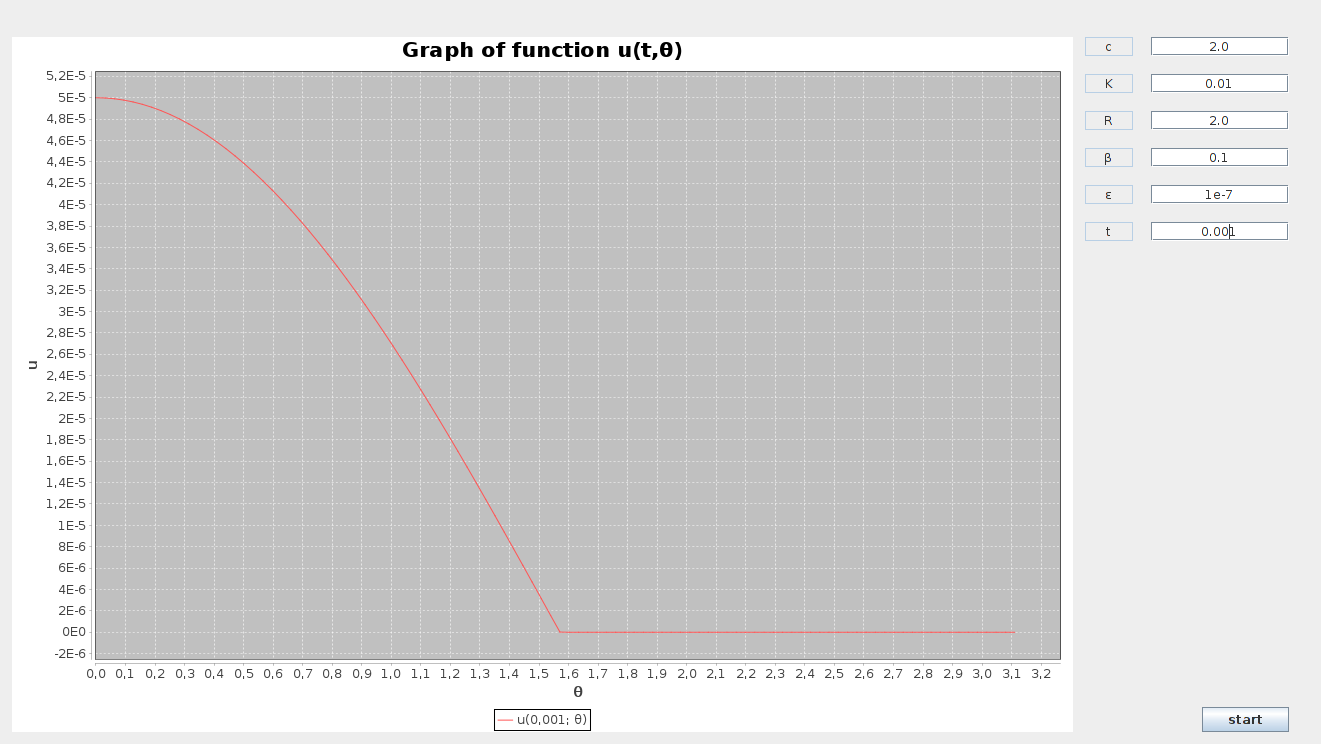
\includegraphics[width=1\linewidth]{screen_t0p001.png}
		\caption{График с исходными значениями при $t=0.001$}
		\label{fig: screen_t0p001}
	\end{center}
	\end{figure}
	\begin{figure}[h]
	\begin{center}
		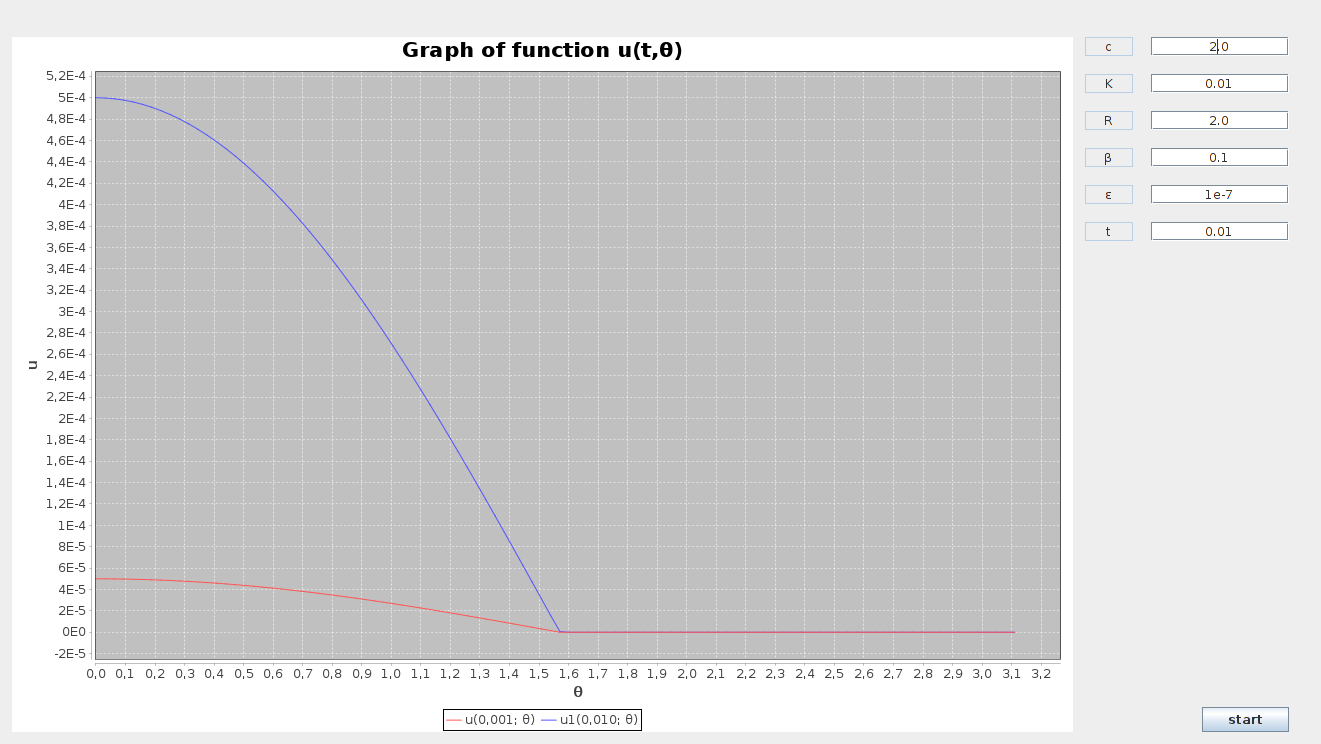
\includegraphics[width=1\linewidth]{screen_t0p01.png}
		\caption{График после изменения $t$ на $0.01$}
		\label{fig: screen_t0p001}
	\end{center}
	\end{figure}
	\begin{figure}[h]
	\begin{center}
		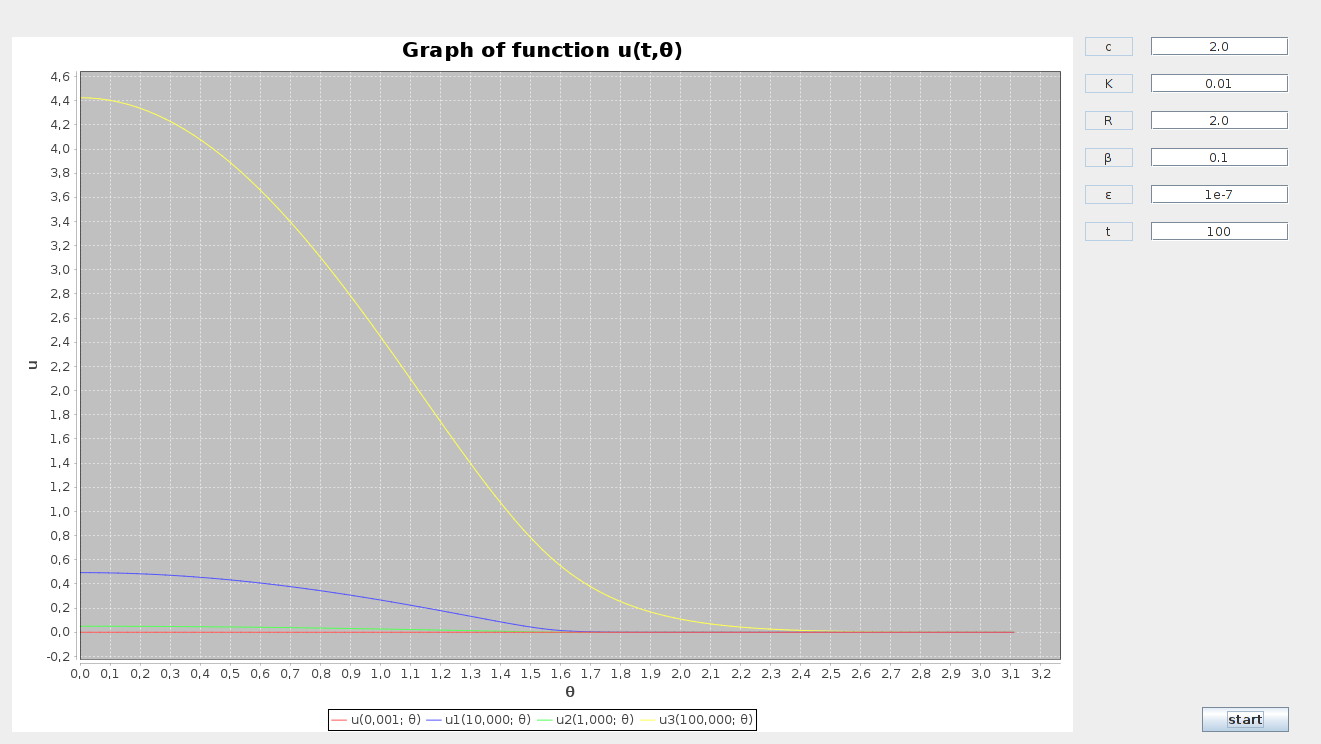
\includegraphics[width=1\linewidth]{screen_dif_t.png}
		\caption{Графики при различных $t\geqslant 0.001$}
		\label{fig: screen_t0p001}
	\end{center}
	
	\end{figure}
	\begin{figure}[h]
	\begin{center}
		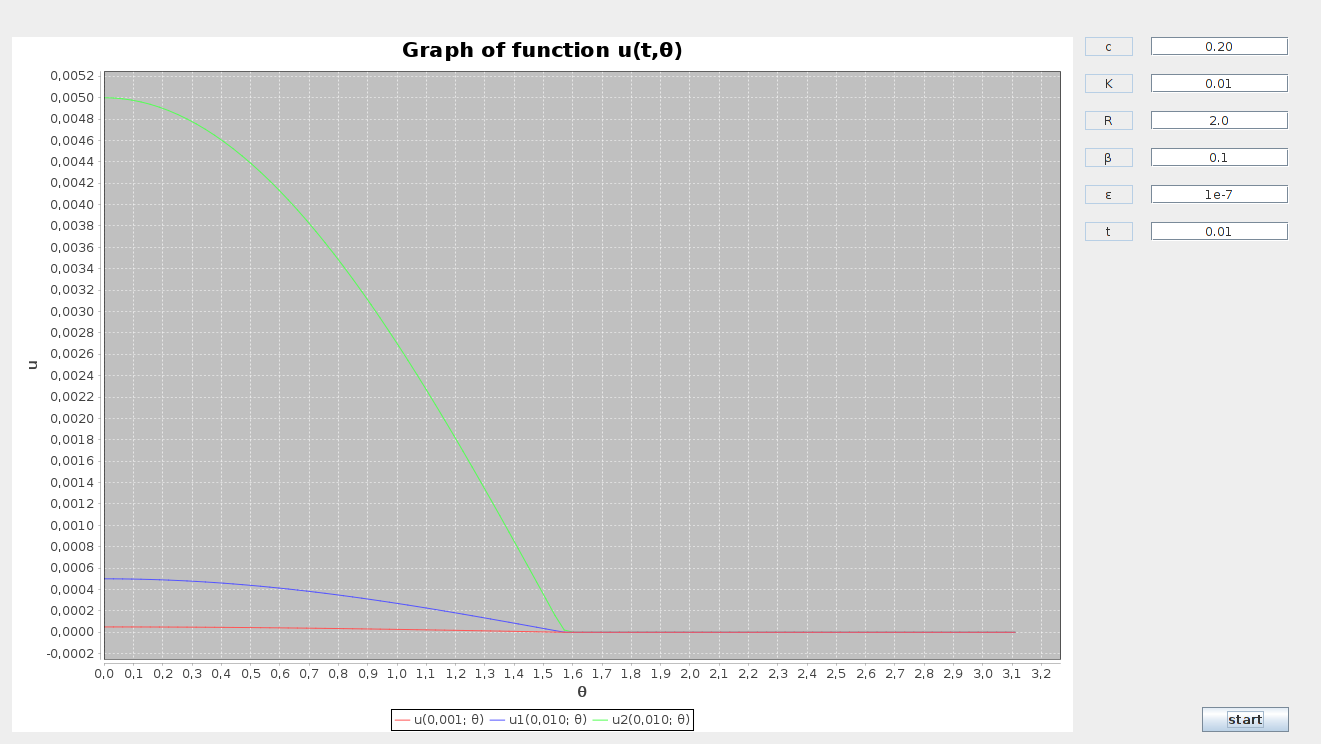
\includegraphics[width=1\linewidth]{screen_c0p2.png}
		\caption{График после изменения $c$ на $0.2$}
		\label{fig: screen_t0p001}
	\end{center}
	\end{figure}
%%\lstset{ framexleftmargin=8mm, tabsize=3, frame=shadowbox, rulesepcolor=\color{blue},escapechar=@}
\section*{Приложение А.}
\begin{center}
{\normalsize \textbf{\textsc{исходный код программы}}}
\end{center}
\addcontentsline{toc}{section}{Приложение А.  Исходный код программы}
\lstinputlisting[language=scala, mathescape, numbers=left]{/home/misha/F.cpp}
	\section*{Заключение}
% http://tex.stackexchange.com/questions/74439/table-of-contents-incorrect-page-numbering
\phantomsection
\addcontentsline{toc}{section}{Заключение}
\label{sec:final}
По результатам данной курсовой работы были выполнены следующие задачи:
\begin{itemize}
	\item получено решение задачи математической физики в виде ряда по функциям Лежандра;
	\item исследована сходимость ряда в $L_1$, получена оценка остатка ряда;
	\item разработана программа расчёта решения задачи с требуемой точностью;
	\item с использованием вычислительного эксперимента, исследовано качество полученной аналитической оценки остатка ряда.
\end{itemize}

Таким образом, достигнута цель курсовой работы. 
	% Зачем: Изменение надписи для списка литературы
% Почему: Пункт 2.8.1 Требований по оформлению пояснительной записки.
\renewcommand{\bibsection}{\sectioncentered*{Cписок использованных источников}}
\phantomsection\pagebreak% исправляет нумерацию в документе и исправляет гиперссылки в pdf
%\renewcommand{\bibnumfmt}[1]{#1}
%\bibliographystyle{gost2008}
\bibliography{emfWork}	 	  	
\end{document}